\documentclass[tikz,border=8pt]{standalone}
% Shared look for every TikZ diagram. Load with % Shared look for every TikZ diagram. Load with % Shared look for every TikZ diagram. Load with \input{../../tools/tikz-style.tex}
\usepackage[T1]{fontenc}
\usepackage{lmodern}
\renewcommand{\sfdefault}{lmr}  % diagrams use the same serif as the text
\usetikzlibrary{arrows.meta, positioning, shapes.geometric, calc, fit, backgrounds}
\definecolor{cblue}{HTML}{4C78A8}
\definecolor{corange}{HTML}{F58518}
\definecolor{cgreen}{HTML}{54A24B}
\definecolor{cred}{HTML}{E45756}
\definecolor{cpurple}{HTML}{B279A2}
\definecolor{cgrey}{HTML}{6B6B6B}
\tikzset{
  every picture/.style={font=\sffamily, line width=1.2pt},
  box/.style={draw=#1, fill=#1!12, rounded corners=4pt, align=center, inner sep=7pt, minimum height=1.1cm},
  box/.default=cgrey,
  arrow/.style={-{Stealth[length=3mm]}, draw=cgrey, line width=1.4pt},
  title/.style={font=\sffamily\bfseries\Large},
  note/.style={font=\sffamily\small, text=cgrey, align=center},
}
\AtBeginDocument{\hyphenpenalty=10000 \exhyphenpenalty=10000}

\usepackage[T1]{fontenc}
\usepackage{lmodern}
\renewcommand{\sfdefault}{lmr}  % diagrams use the same serif as the text
\usetikzlibrary{arrows.meta, positioning, shapes.geometric, calc, fit, backgrounds}
\definecolor{cblue}{HTML}{4C78A8}
\definecolor{corange}{HTML}{F58518}
\definecolor{cgreen}{HTML}{54A24B}
\definecolor{cred}{HTML}{E45756}
\definecolor{cpurple}{HTML}{B279A2}
\definecolor{cgrey}{HTML}{6B6B6B}
\tikzset{
  every picture/.style={font=\sffamily, line width=1.2pt},
  box/.style={draw=#1, fill=#1!12, rounded corners=4pt, align=center, inner sep=7pt, minimum height=1.1cm},
  box/.default=cgrey,
  arrow/.style={-{Stealth[length=3mm]}, draw=cgrey, line width=1.4pt},
  title/.style={font=\sffamily\bfseries\Large},
  note/.style={font=\sffamily\small, text=cgrey, align=center},
}
\AtBeginDocument{\hyphenpenalty=10000 \exhyphenpenalty=10000}

\usepackage[T1]{fontenc}
\usepackage{lmodern}
\renewcommand{\sfdefault}{lmr}  % diagrams use the same serif as the text
\usetikzlibrary{arrows.meta, positioning, shapes.geometric, calc, fit, backgrounds}
\definecolor{cblue}{HTML}{4C78A8}
\definecolor{corange}{HTML}{F58518}
\definecolor{cgreen}{HTML}{54A24B}
\definecolor{cred}{HTML}{E45756}
\definecolor{cpurple}{HTML}{B279A2}
\definecolor{cgrey}{HTML}{6B6B6B}
\tikzset{
  every picture/.style={font=\sffamily, line width=1.2pt},
  box/.style={draw=#1, fill=#1!12, rounded corners=4pt, align=center, inner sep=7pt, minimum height=1.1cm},
  box/.default=cgrey,
  arrow/.style={-{Stealth[length=3mm]}, draw=cgrey, line width=1.4pt},
  title/.style={font=\sffamily\bfseries\Large},
  note/.style={font=\sffamily\small, text=cgrey, align=center},
}
\AtBeginDocument{\hyphenpenalty=10000 \exhyphenpenalty=10000}

\usetikzlibrary{matrix}
\begin{document}
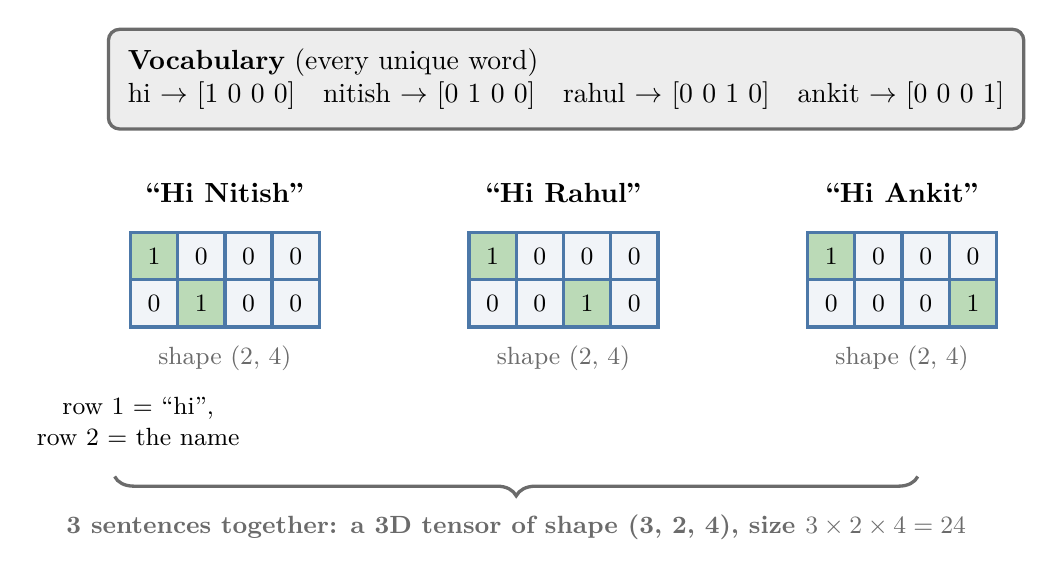
\begin{tikzpicture}
  \tikzset{oh/.style={matrix of nodes, ampersand replacement=\&, column sep=-\pgflinewidth, row sep=-\pgflinewidth,
      nodes={minimum size=0.6cm, anchor=center, draw=cblue, fill=cblue!8, font=\small}}}
  % vocabulary
  \node[box=cgrey, align=left, anchor=north west] (vocab) at (-0.3,3.4) {\textbf{Vocabulary} (every unique word)\\
    hi $\rightarrow$ [1 0 0 0]\quad nitish $\rightarrow$ [0 1 0 0]\quad rahul $\rightarrow$ [0 0 1 0]\quad ankit $\rightarrow$ [0 0 0 1]};
  \foreach \s/\w/\c [count=\i] in {Hi Nitish/nitish/2, Hi Rahul/rahul/3, Hi Ankit/ankit/4} {
    \pgfmathsetmacro{\x}{(\i-1)*4.3}
    \node[font=\bfseries] at (\x+1.2,1.3) {``\s''};
    \matrix (m\i) [oh] at (\x+1.2,0.2) {
      |[fill=cgreen!40]| 1 \& 0 \& 0 \& 0 \\
      0 \& 0 \& 0 \& 0 \\ };
    \node[note] at (\x+1.2,-0.8) {shape (2, 4)};
  }
  \node[fill=cgreen!40, draw=cblue, minimum size=0.6cm, font=\small] at (m1-2-2) {1};
  \node[fill=cgreen!40, draw=cblue, minimum size=0.6cm, font=\small] at (m2-2-3) {1};
  \node[fill=cgreen!40, draw=cblue, minimum size=0.6cm, font=\small] at (m3-2-4) {1};
  \node[note, text=black, align=center] at (0.1,-1.6) {row 1 = ``hi'',\\row 2 = the name};
  \draw[decorate, decoration={brace, amplitude=7pt, mirror}, cgrey] (-0.2,-2.3) -- (10.0,-2.3)
    node[midway, below=10pt, font=\small\bfseries] {3 sentences together: a 3D tensor of shape (3, 2, 4), size $3 \times 2 \times 4 = 24$};
\end{tikzpicture}
\end{document}
